%%%%%%%%%%%%%%%%%%%%%%%%%%%%%%%%%%%%%%%%%%%%%%%%%%%%%%%%%%%%%%%%%%%%%%%%%%%%%%%%
%%%%%%%%%%%%%%%%%%%%%%%%%%%%%%%%%%%%%%%%%%%%%%%%%%%%%%%%%%%%%%%%%%%%%%%%%%%%%%%%
\documentclass[addpoints,12pt,solution]{exam}
\printanswers
\usepackage{amsmath,amssymb}
\usepackage{comment}
\usepackage{graphicx}
\usepackage{ulem}
\usepackage{paralist}
\usepackage{psfrag}
\usepackage{fullpage}
\usepackage{fancybox}
\usepackage{ifthen}
\usepackage{hyperref}
\usepackage{marvosym}
\usepackage{amsmath}
\usepackage{float}
\usepackage{tikz}

\DeclareMathOperator*{\argmax}{arg\,max}
\DeclareMathOperator*{\argmin}{arg\,min}
\DeclareMathOperator*{\real}{\mathbb{R}}
\usepackage{enumitem}
\usepackage{algorithm}
\usepackage{algpseudocode}
\marksnotpoints


\begin{document}


\hrule
\vspace{1mm}
\noindent 
\begin{center}
{\Large CS6700 : Reinforcement Learning} \\
{\large Written Assignment \#1}
\end{center}
\vspace{1mm}
\noindent 
{\textbf{Topics}: Intro, Bandits, MDP, Q-learning, SARSA, FA, DQN \hfill \textbf{Deadline}: 20/03/2024, 23:55}\\


%%%%%%%%%%%%%%%%%%%%%%%%%%%%%%%%%%%%%%%%%%%%%%%%%%%%%%%%%%%%%%%%
% Enter name and roll number here
\noindent {\bf Name: }--Your name here--  \hfill {\bf Roll number: }--Your roll no. here-- 
%%%%%%%%%%%%%%%%%%%%%%%%%%%%%%%%%%%%%%%%%%%%%%%%%%%%%%%%%%%%%%%%%%
\vspace{2mm}
\hrule

{\small

\begin{itemize}\itemsep0mm
\item This is an individual assignment. Collaborations and discussions are strictly
prohibited.
\item Be precise with your explanations. Unnecessary verbosity will be penalized.
\item Check the Moodle discussion forums regularly for updates regarding the assignment.
\item Type your solutions in the provided \LaTeX template file.
\item \textbf{Please start early.}
\end{itemize}
}

\hrule

\vspace{3mm}




%\gradetable[h][questions]

%%%%%%%%%%%%%%%%%%%%%%%%%%%%%%%%%%%%%%%%%%%%%%%%%%%%%%%%%%%%%%%%%%%%%%%%%%%%%%
%%%%%%%%%%%%%%%%%%%%%%%%%%%%%%%START HERE%%%%%%%%%%%%%%%%%%%%%%%%%%%%%%%%%%%%%%
\begin{questions}

\question[3][TD, IS] Consider the following deterministic grid-world. 

\begin{figure}[!htp]
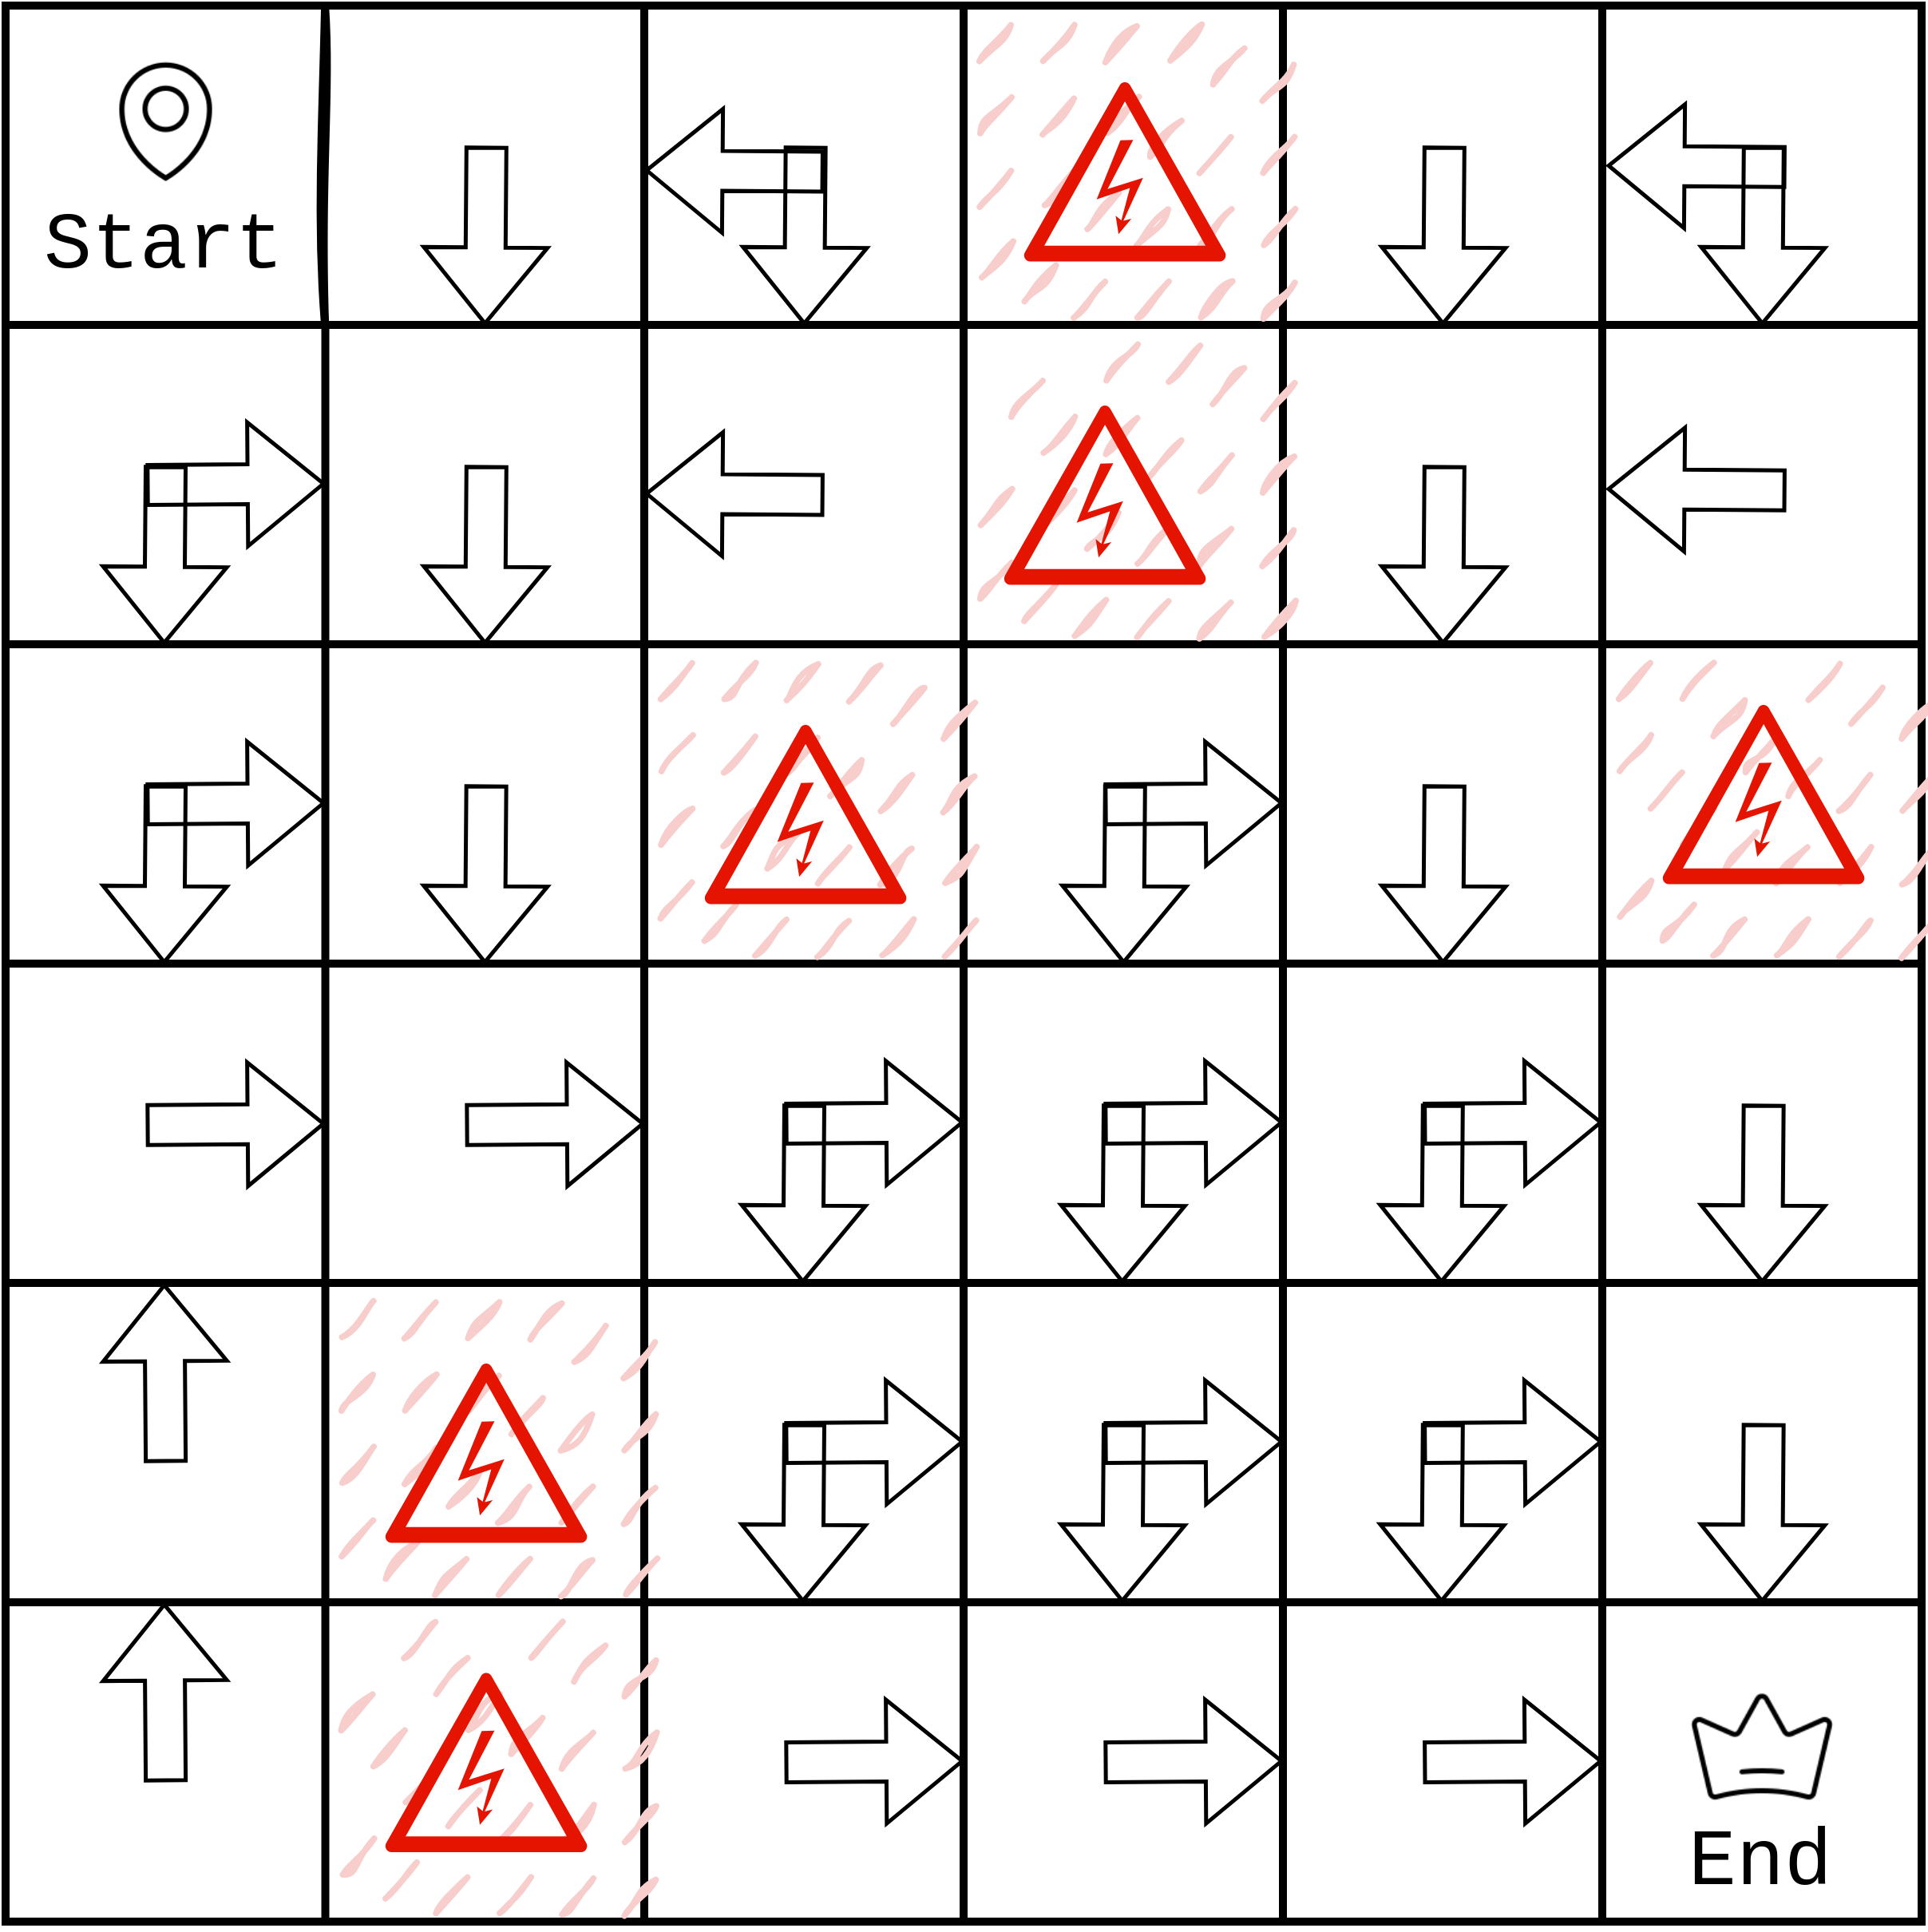
\includegraphics[width=0.35\textwidth]{2024/WA1/gridworld.png}\centering
\end{figure}

 
Every actions yields a reward of -1 and landing in the red-danger states yields an additional -5 reward. The optimal policy is represented by the arrows. Now, can you learn a value function of an arbitrary policy while strictly following the optimal policy? Support your claim.


\begin{solution}

\end{solution}

\question[1][SARSA] In a 5 x 3 cliff-world two versions of SARSA are trained until convergence. The sole distinction between them lies in the $\epsilon$ value utilized in their $\epsilon$-greedy policies. Analyze the acquired optimal paths for each variant and provide a comparison of their $\epsilon$ values, providing a justification for your findings.

\begin{figure}[!htp]
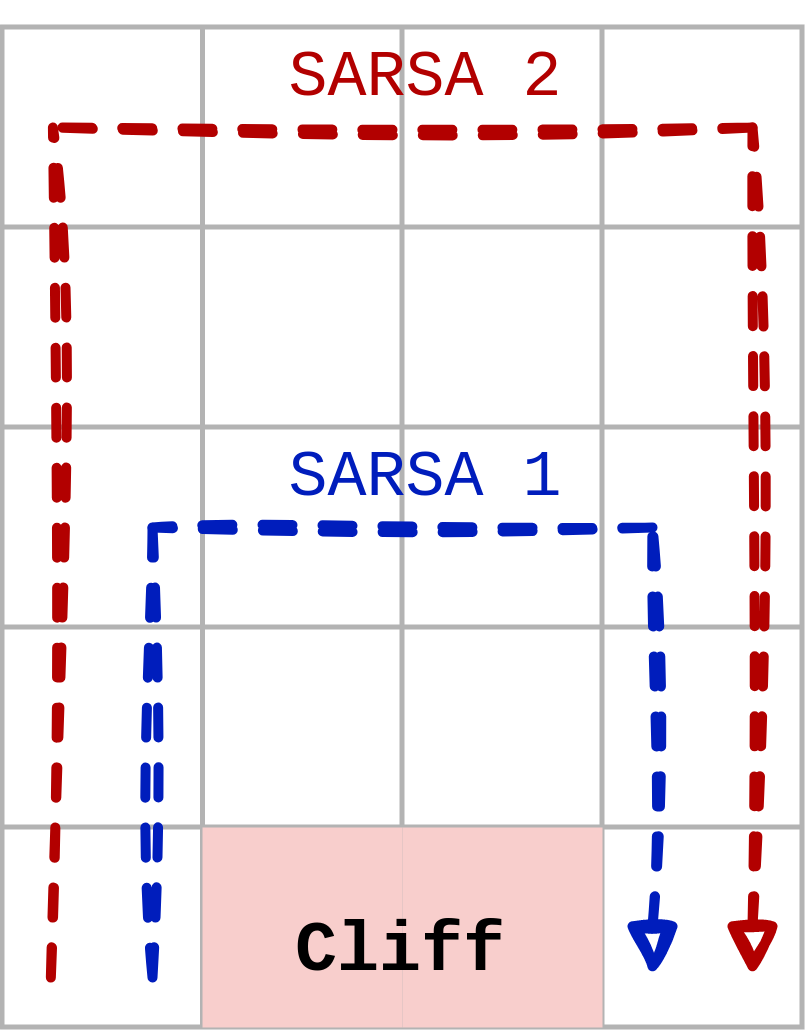
\includegraphics[width=0.25\textwidth]{2024/WA1/cliff_walking.png}\centering
\end{figure}

\begin{solution}

\end{solution}

\question[2][SARSA] The following grid-world is symmetric along the dotted diagonal. Now, there exists a symmetry function $F:S \times A \rightarrow S \times A$, which maps a state-action pair to its symmetric equivalent. For instance, the states $S_1$ and $S_2$ are symmetrical and \\ F($S_1$,North) = $S_2$,East.

\begin{figure}[!htp]
\centering 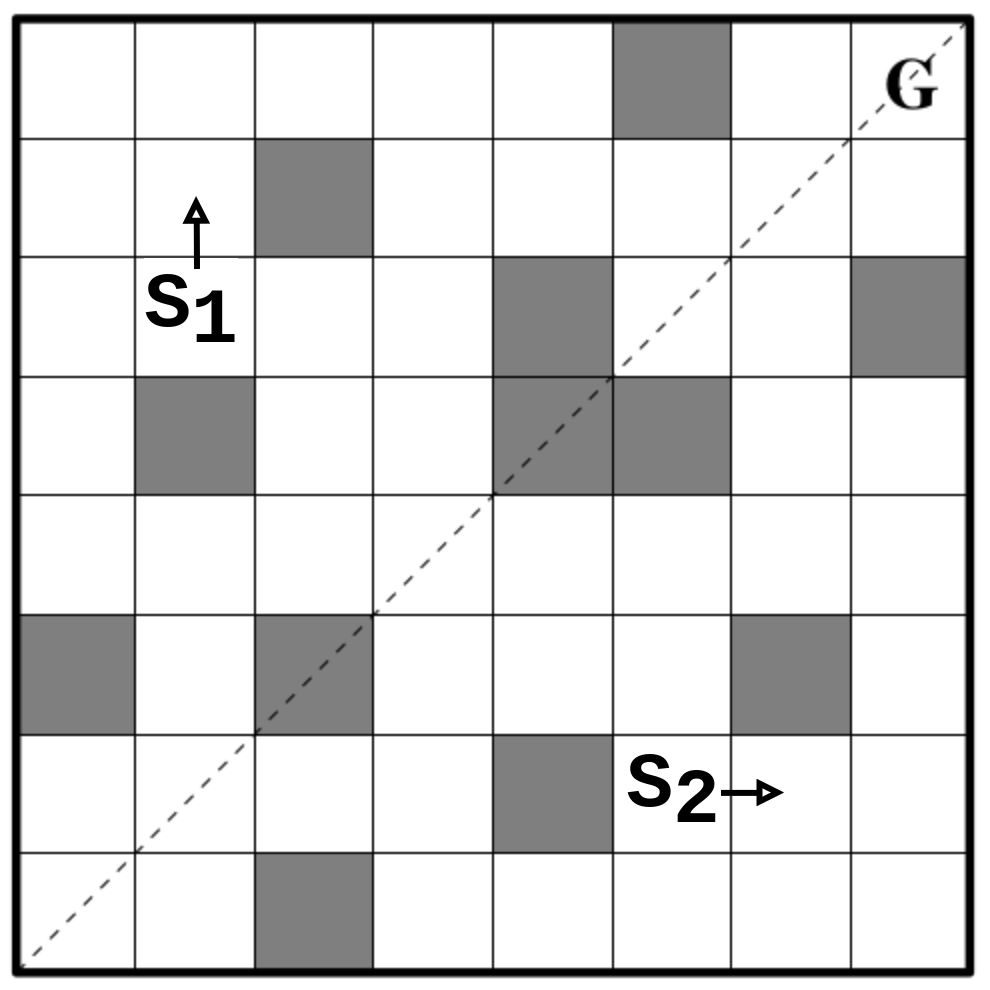
\includegraphics[width=.3\textwidth]{2024/WA1/symmetry_world.png}
\end{figure}

Given the standard SARSA pseudo-code below, how can the pseudo-code be adapted to incorporate the symmetry function $F$ for efficient learning?

\begin{algorithm}[H]
\caption{SARSA Algorithm}
\begin{algorithmic}
    \State Initialize $Q$-values for all state-action pairs arbitrarily
    \For {each episode}
        \State Initialize state $s$
        \State Choose action $a$ using $\epsilon$-greedy policy based on $Q$-values
        \While {not terminal state}
            \State Take action $a$, observe reward $r$ and new state $s'$
            \State Choose action $a'$ using $\epsilon$-greedy policy based on $Q$-values for state $s'$
            \State $Q(s, a) \gets Q(s, a) + \alpha \left( r + \gamma Q(s', a') - Q(s, a) \right)$
            \State $s \gets s'$, $a \gets a'$
        \EndWhile
    \EndFor
\end{algorithmic}
\end{algorithm}

\begin{solution}

\end{solution}

\question[4][VI] Consider the below deterministic MDP with $N$ states. At each state there are two possible actions, each of which deterministically either takes you to the next state or leaves you in the same state. The initial state is $1$ and consider a shortest path setup to state $N$ (Reward -1 for all transitions except when terminal state $N$ is reached). 
\begin{center}
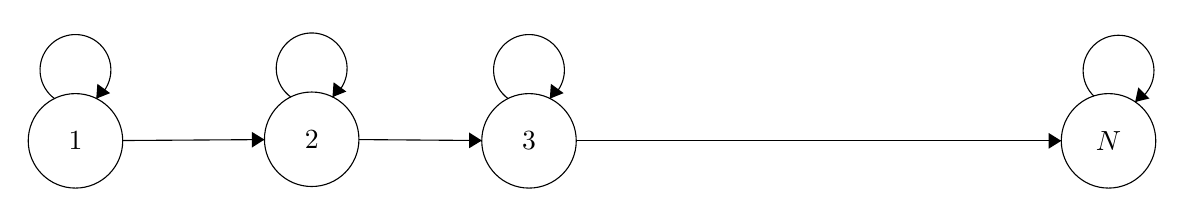
\begin{tikzpicture}[scale=0.2]
\tikzstyle{every node}+=[inner sep=0pt]
\draw [black] (3.3,-7.1) circle (3);
\draw (3.3,-7.1) node {$1$};
\draw [black] (18.3,-7) circle (3);
\draw (18.3,-7) node {$2$};
\draw [black] (32.1,-7.1) circle (3);
\draw (32.1,-7.1) node {$3$};
\draw [black] (68.9,-7.1) circle (3);
\draw (68.9,-7.1) node {$N$};
\draw [black] (6.3,-7.08) -- (15.3,-7.02);
\fill [black] (15.3,-7.02) -- (14.5,-6.53) -- (14.5,-7.53);
\draw [black] (21.3,-7.02) -- (29.1,-7.08);
\fill [black] (29.1,-7.08) -- (28.3,-6.57) -- (28.3,-7.57);
\draw [black] (35.1,-7.1) -- (65.9,-7.1);
\fill [black] (65.9,-7.1) -- (65.1,-6.6) -- (65.1,-7.6);
\draw [black] (1.977,-4.42) arc (234:-54:2.25);
\fill [black] (4.62,-4.42) -- (5.5,-4.07) -- (4.69,-3.48);
\draw [black] (16.977,-4.32) arc (234:-54:2.25);
\fill [black] (19.62,-4.32) -- (20.5,-3.97) -- (19.69,-3.38);
\draw [black] (30.777,-4.42) arc (234:-54:2.25);
\fill [black] (33.42,-4.42) -- (34.3,-4.07) -- (33.49,-3.48);
\draw [black] (67.97,-4.26) arc (225.8659:-62.1341:2.25);
\fill [black] (70.59,-4.63) -- (71.5,-4.41) -- (70.79,-3.71);
\end{tikzpicture}
\end{center}
Now on applying the following Value Iteration algorithm on this MDP, answer the below questions:

\begin{algorithm}
\caption{Value Iteration Algorithm}
\begin{algorithmic}[1]
    \State Initialize $V$-values for all states arbitrarily over the state space $S$ of $N$ states. Define a permutation function $\phi$ over the state space
    \State $i \xleftarrow[]{} 0$
    \While{\text{NotOptimal(V)}}
    \State $s \xleftarrow[]{} \phi(i \mod N)$
    \State $V(s) \xleftarrow[]{} \max_a \sum_{s, r'} p(s', r|s, a)[r + \gamma*V(s')]$
    \State $i \xleftarrow{} i + 1$
    \EndWhile

\end{algorithmic}
\end{algorithm}
\begin{enumerate}
    \item (1 mark) Design a permutation function $\phi$ (which is a one-one mapping from the state space to itself, defined \href{https://en.wikipedia.org/wiki/Permutation#Definition}{here}), such that the VI algorithm converges the fastest and reason about how many steps (value of $i$) it would take.
    \begin{solution}
        
    \end{solution}
    \item (1 mark) Design a permutation function $\phi$ such that the VI algorithm would take the most number of steps to converge to the optimal solution and again reason how many steps that would be.
    \begin{solution}
        
    \end{solution}
    \item (2 marks) 
    Finally, in a realistic setting, there is often no known semantic meaning associated with the numbering over the sets and a common strategy is to randomly sample a state from $S$ every timestep. Performing the above algorithm with $s$ being a randomly sampled state, what is the expected number of steps the algorithm would take to converge?
    \begin{solution}
        
    \end{solution}
    \textbf{Note:} Do not worry about exact constants/one-off differences, as long as the asymptotic solution is correct with the right reasoning, full marks will be given. 
\end{enumerate}

\question[5] [TD, MC] Suppose that the system that you are trying to learn about (estimation or control) is not perfectly Markov. Comment on the suitability of using different solution approaches for such a task, namely, Temporal Difference learning, Monte Carlo methods. Explicitly state any assumptions that you are making.
\begin{solution}

\end{solution}

\question[6][MDP] Consider the continuing MDP shown below. The only decision
to be made is that in the \textit{top} state (say, $s_0$), where two actions are
available, \textit{left} and \textit{right}. The numbers show the rewards that are
received deterministically after each action. There are exactly two
deterministic policies, $\pi_{left}$ and $\pi_{right}$. Calculate and show which
policy will be the optimal:
\begin{figure}[!htp]
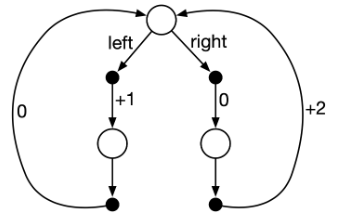
\includegraphics[width=0.4\textwidth]{2024/WA1/MDP_Q10.png}\centering
\end{figure}
\begin{enumerate}[label=(\alph*)]
    \item (2 marks) if $\gamma = 0$
    \begin{solution}
        
    \end{solution}
    \item (2 marks) if $\gamma = 0.9$
    \begin{solution}
        
    \end{solution}
    \item (2 marks) if $\gamma = 0.5$
    \begin{solution}
        
    \end{solution}
\end{enumerate}


\question[3] Recall the three advanced value-based methods we studied in class: Double DQN, Dueling DQN, Expected SARSA.
While solving some RL tasks, you encounter the problems given below. Which advanced value-based method would you use to overcome it and why? Give one or two lines of explanation for `why’.
\begin{enumerate}[label=(\alph*)]
    \item (1 mark) Problem 1: In most states of the environment, choice of action doesn’t matter.
    \begin{solution}

    \end{solution}
    \item (1 mark) Problem 2: Agent seems to be consistently picking sub-optimal actions during exploitation.
    \begin{solution}
 
    \end{solution}
    \item (1 mark) Problem 3: Environment is stochastic with high negative reward and low positive reward, like in cliff-walking.
    \begin{solution}
    
    \end{solution}
\end{enumerate}

\question[2][REINFORCE] Recall the update equation for \textit{preference} ${H_t}(a)$ for all arms. 
\begin{equation*}
    {H_{t+1}}(a) =
    \begin{cases} 
        {H_t}(a) + {\alpha}\left({R_t} - K\right)\left(1 - {\pi_t}(a)\right) \; \text{if} \: a = {A_t} \\
        {H_t}(a) + {\alpha}\left({R_t} - K\right){\pi_t}(a) \quad\quad\quad  \text{if} \: a \neq {A_t}
    \end{cases}
\end{equation*}
\noindent where ${\pi_t}(a) = {e^{{H_t}(a)}}/{\sum_b e^{{H_t}(b)}}$. Here, the quantity $K$ is chosen to be $\bar{R_t} = \left({\sum_{s=1}^{t-1} {R_s}}\right)/{t-1}$ because it empirically works. Provide concise explanations to these following questions. Assume all the rewards are non-negative.

\begin{enumerate}[label=(\alph*)]
    \item (1 mark) How would the quantities $\{{{\pi_t}(a)}\}_{a \in \mathcal{A}}$ be affected if $K$ is chosen to be a large positive scalar? Describe the policy it converges to.
    \begin{solution}
        
    \end{solution}
    \item (1 mark) How would the quantities $\{{{\pi_t}(a)}\}_{a \in \mathcal{A}}$ be affected if $K$ is chosen to be a small positive scalar? Describe the policy it converges to.
    \begin{solution}
        
    \end{solution}
\end{enumerate}

\question[3][Delayed Bandit Feedback] Provide pseudocodes for the following MAB problems. Assume all arm rewards are gaussian.
\begin{enumerate}[label=(\alph*)]
    \item (1 mark) UCB algorithm for a stochastic MAB setting with arms indexed from $0$ to $K-1$ where $K \in \mathbb{Z}^+$.
    \begin{solution}
        
    \end{solution}
    \item (2 marks) Modify the above algorithm so that it adapts to the setting where agent observes a feedback tuple instead of reward at each timestep. The feedback tuple $h_t$ is of the form $({t'}, {r_{t'}})$ where ${t'} \sim \text{Unif}(\max(t-m+1, 1), t)$, $m \in {\mathbb{Z}^+}$ is a constant, and ${r_{t'}}$ represents the reward obtained from the arm pulled at timestep $t'$. 
    \begin{solution}
        
    \end{solution}
\end{enumerate}

\question[6][Function Approximation] Your are given an MDP, with states $s_1$, $s_2$, $s_3$ and actions $a_1$ and $a_2$. Suppose the states $s$ are represented by two features, $\Phi_1(s)$ and $\Phi_2(s)$, where $\Phi_1(s_1) = 2$, $\Phi_1(s_2) = 4$, $\Phi_1(s_3) = 2$, $\Phi_2(s_1) = -1$, $\Phi_2(s_2)=0$ and $\Phi_2(s_3)=3$.
\begin{enumerate}
    \item (3 marks) What class of state value functions can be represented using only these features in a linear function approximator? Explain your answer.
    \begin{solution}
        
    \end{solution}
    \item (3 marks) Updated parameter weights using gradient descent TD(0) for experience given by: $s_2, a_1, -5, s_1$. Assume state-value function is approximated using linear function with initial parameters weights set to zero and learning rate $0.1$.
    \begin{solution}
        
    \end{solution}
\end{enumerate}

\end{questions}
%%%%%%%%%%%%%%%%%%%%%%%%%%%%%%%%%%%%%%THE END%%%%%%%%%%%%%%%%%%%%%%%%%%%%%%%%%%%

\end{document}